\section{The Value Frontier: Cost, Quality, and Speed}
\label{sec:frontier}

A leaderboard ranked on quality alone answers ``which model is best'' but not the
question a deploying team actually faces: \emph{best per dollar, and per second}.
A frontier model that wins a deal at ten times the token cost and three times the
latency of a mid-tier model is not obviously the right choice for an agent that
must run thousands of live sales cycles. We therefore report VEB not as a single
ranking but as a \emph{Value Frontier}: the Pareto surface over sale quality, cost,
and speed, on which each model is a point and only the non-dominated models form
the front.

\subsection{Measuring cost}
Cost is not estimated; it is measured per cell. Every trajectory records the exact
input and output token counts and the realized USD cost of every model call, priced
at each provider's public per-token rates. Aggregated to the completed-deal level,
this yields a \textbf{cost-per-completed-deal} for each model that is authoritative
rather than inferred---the strongest form of the axis, because it is our own ground
truth and requires no external reconstruction. Across the roster, cost-per-deal
spans roughly \resCostPerDealMin{}--\resCostPerDealMax{}~USD, a range wide enough
that it, not quality, dominates the deployment decision for many use cases.

Two caveats keep this axis honest. First, cost-per-deal divides total spend by the
number of \emph{clean wins}, and for low-win models that denominator is small (the
\$\resCostPerDealMax{} figure rests on 11 wins), so the per-deal point estimates
for weak closers are noisy. We therefore also report the denominator-free
\textbf{cost-per-run}: pooled across both tracks it spans \$0.39
(gemini-3.5-flash) to \$23.62 (claude-fable-5) per episode---a $\sim$60$\times$
spread---with the frontier leader \resFrontierBest{} at \$1.00 per run. Second,
list pricing for \texttt{gpt-5.6-sol} and \texttt{grok-4.5} carries the
provider's adjacent-tier rate pending published prices
(Appendix~\ref{app:models}). Neither caveat threatens the headline: the
cheapest-per-run models are also among the cheapest per deal, and the dominance
of \resFrontierBest{} holds under either denominator.

\subsection{Measuring speed and reliability}
Latency and request reliability are recovered from the gateway through which all
seller, buyer, and judge traffic is routed. Because the gateway persists only the
engagement-level identifier on its aggregation surface, we obtain per-model latency
by grouping the raw request log by the preserved model field, and we report
request-success reliability at the engagement level. Median call latency is
\resLatencyPfifty{}~s and p90 is \resLatencyPninety{}~s, at an engagement-wide reliability
of \resReliability{}\%. We are explicit about the provenance limits of this axis
(Section~\ref{sec:limitations}): cost is per-cell exact, latency is per-model from
the log grouping, and reliability is engagement-wide.

\subsection{The frontier}
Figure~\ref{fig:frontier} plots mean SQS against cost-per-deal on the two axes we
measure per cell exactly; the non-dominated models trace the Value Frontier. The
striking result is how the trade-off collapses: a single model, \resFrontierBest{},
is simultaneously the highest-quality \emph{and} the cheapest-per-deal seller on
the board, delivering \resFrontierBestSQSPerUSD{} SQS points per USD and strictly
dominating every other endpoint on both axes at once. The rest of the story is in
the \emph{spread}: cost-per-deal ranges more than two-hundred-fold across the
roster, from \$\resCostPerDealMin{} to \$\resCostPerDealMax{} per completed deal,
so the expensive models are not buying quality---they are strictly dominated,
paying far more for less. A quality-only leaderboard hides exactly this: that the
best seller is also the cheapest, and that most of the field is Pareto-dominated
on price and quality together.

\begin{figure}[t]
  \centering
  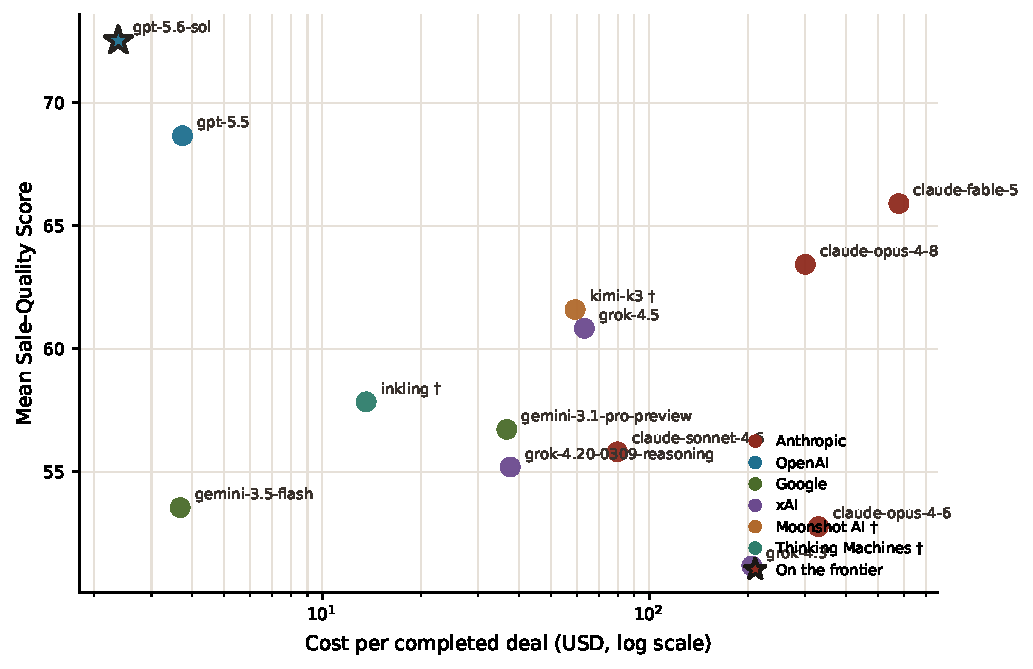
\includegraphics[width=\linewidth]{figures/value_frontier.pdf}
  \caption{The Value Frontier: mean sale quality against cost per completed deal
  (log scale), coloured by lab. Both axes are measured per cell---cost from the
  realized per-token spend, quality from the frozen grades---so the surface is
  ground truth, not reconstruction. The star marks the single non-dominated model:
  \resFrontierBest{} is simultaneously the highest-quality and cheapest-per-deal
  seller on the board. Caveats: per-deal costs for low-win models rest on small
  win counts (the \$\resCostPerDealMax{} point divides by 11 wins);
  \texttt{gpt-5.6-sol} and \texttt{grok-4.5} pricing assumes the provider's
  adjacent-tier list rate. The qualitative conclusion is robust to both: the
  $>200\times$ per-deal spread persists as a $\sim$60$\times$ spread on the
  denominator-free cost-per-run axis.}
  \label{fig:frontier}
\end{figure}
